\subsection{Franke function data}

\subsubsection{Neural network}

Based on the initial search, using the optimizer with momentum seems to be a good choice for further investigation.
Furthermore, we note that the constant optimizer and the RMSprop optimizer make up the best three together with the one with momentum.

\begin{figure}[h!]
    \centering
    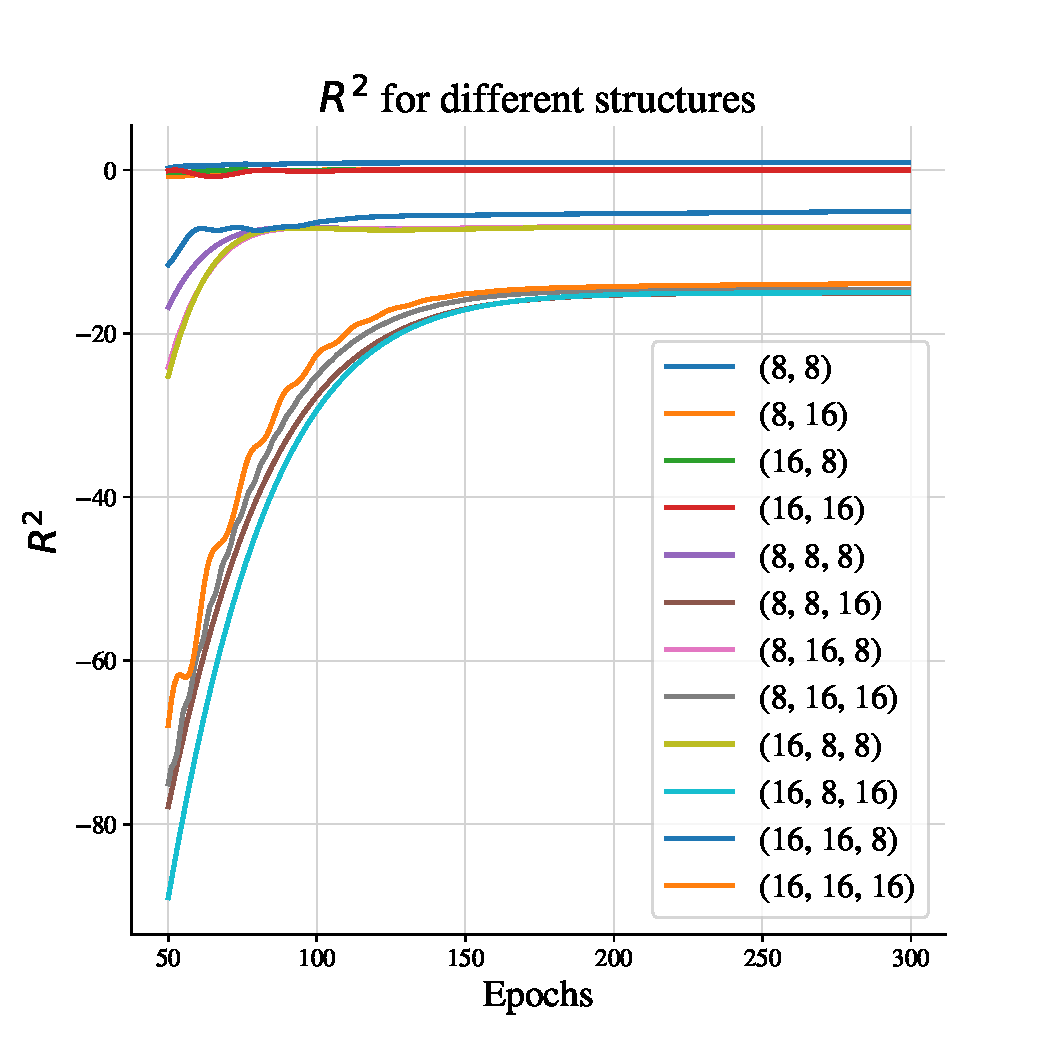
\includegraphics[width=1.0\linewidth]{project_2/figures/$R^2$ for different structures_continuous.pdf}
    \caption{$R^2$ for the neural network for different number of layers and sizes for each layer. The best one is (24,24).}
    \label{fig:structure_franke}
\end{figure}

Fig. \ref{fig:structure_franke} shows the $R^2$ for models with different network structure, but otherwise the same parameters. It is interesting to notice that to layers with a size of 24 each is the model which yields the highest $R^2$ score. We tested for two and three layers and layer sizes of 8 and 24. So it seems fewer but bigger layers are favorable. 
The reason for this might be that \mia{}
The structure of the network dictates \mia{... something about the workings of structure}

\begin{figure}[h!]
    \centering
    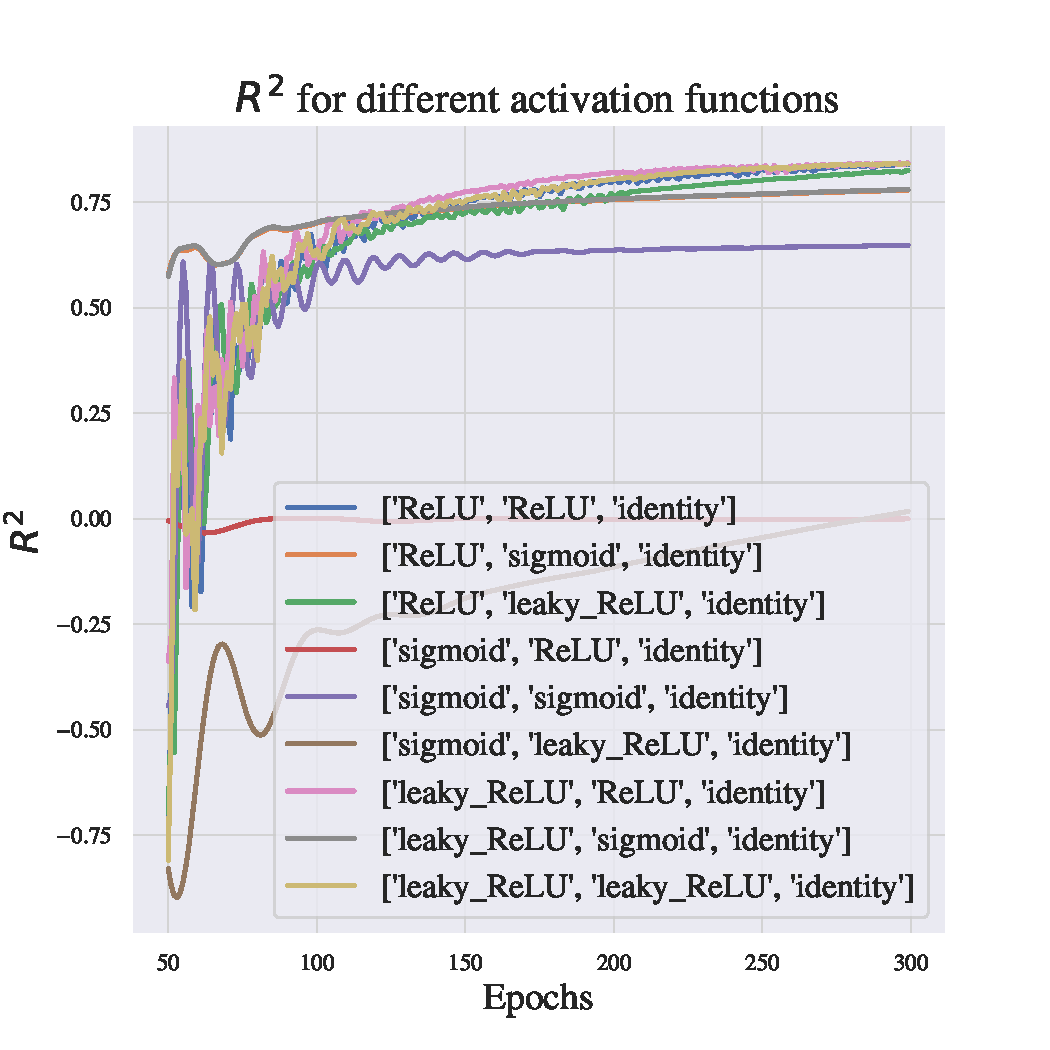
\includegraphics[width=1.0\linewidth]{project_2/figures/$R^2$ for different activation functions_continuous.pdf}
    \caption{The $R^2$ for different choices of activation functions for the two hidden layers. Identity is always used as the final activation function. The best $R^2$ is found when using ReLU at both hidden layers.}
    \label{fig:activation_franke}
\end{figure}

Using the network structure found in the previous step, we try different activation functions for the two hidden layers. 
Fig. \ref{fig:activation_franke} visualizes how the different models perform. 
The three worst performing models are those with sigmoid as the activation function at the first hidden layer. \mia{comment on this}
The four best ones are the ones that combines leaky ReLU and ReLU (both orders) and just one or the other. 
The very best model has ReLU at both hidden layers. 
\mia{more}

\begin{figure}[h!]
    \centering
    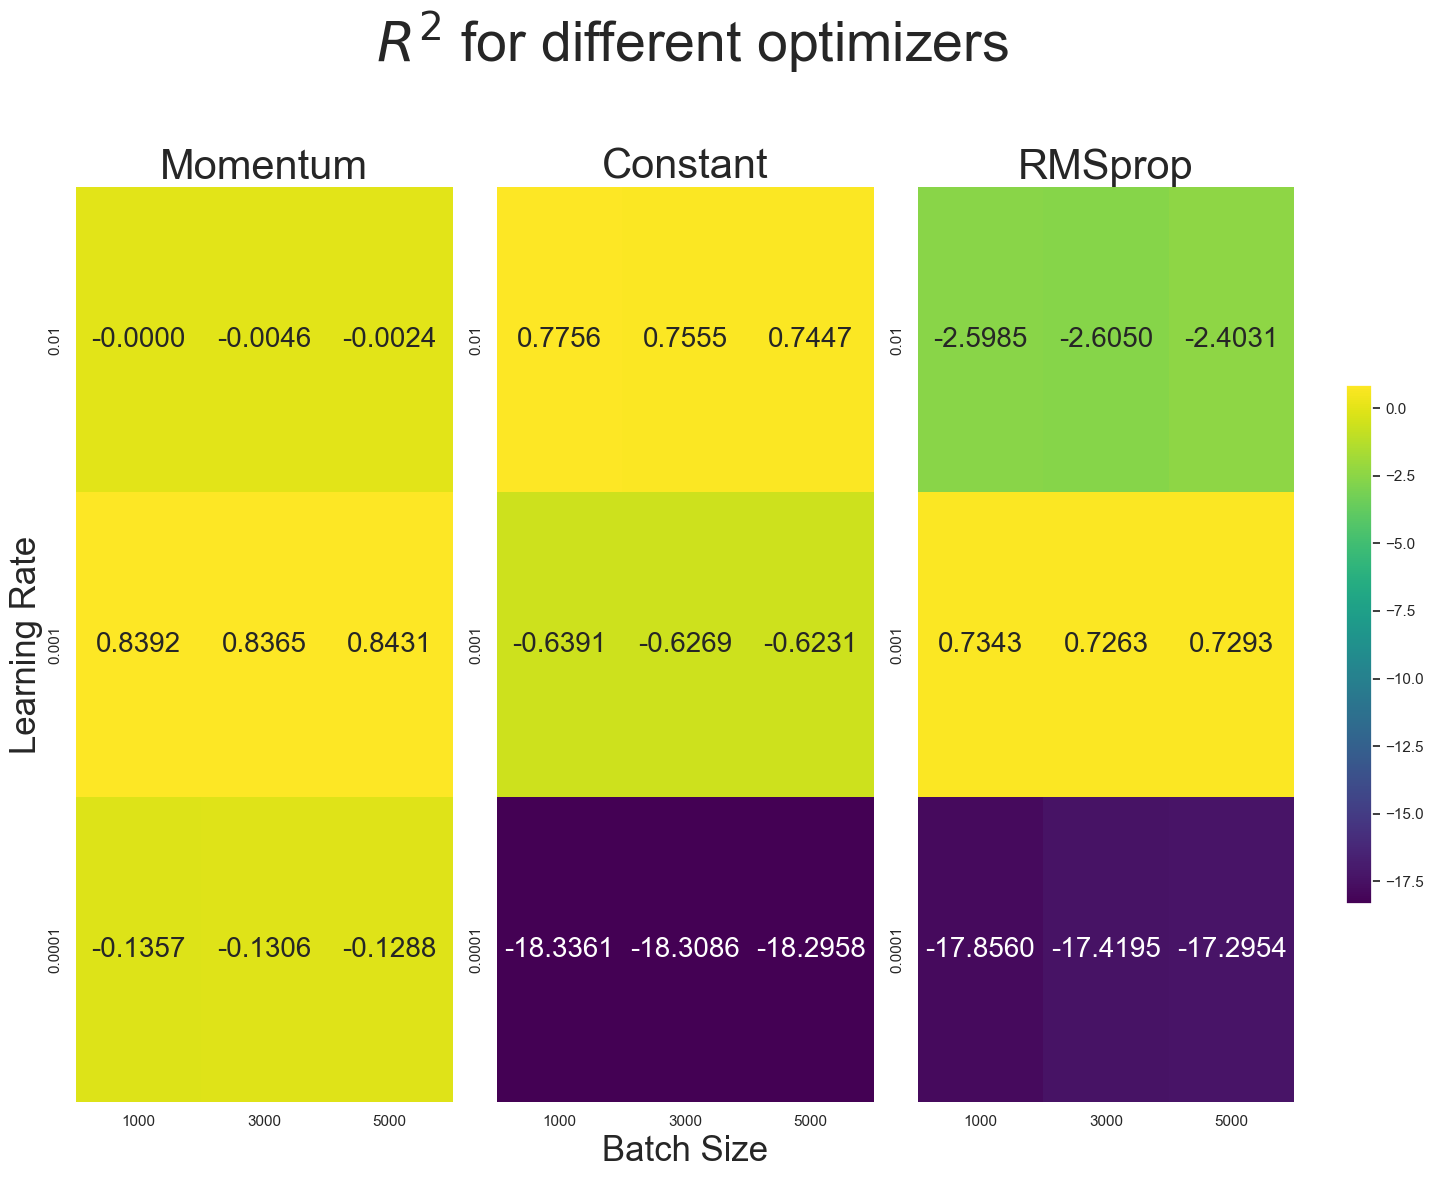
\includegraphics[width=1.0\linewidth]{project_2/figures/r2_grid_cont.png}
    \caption{The $R^2$ on the test set for different sets of learning rates and batch sizes for the three best optimizers.}
    \label{fig:grid_franke}
\end{figure}

Using (2,24,24,1) as the network structure and (ReLU, ReLU, identity) as the activation functions, the grid search for the best combination of initial learning rate and batch size is shown in Fig. \ref{fig:grid_franke}. The three best optimizers, constant, with momentum, and RMSprop, are used. 
We look for the combination that gives the highest $R^2$on the test set for each of the optimizers. 

The momentum and RMSprop optimizer makes an adjustment to this learning rate as the training progresses. It seems starting with too high of a value, gives a very slow convergence. For the constant \mia{more}

The best combination of learning rate and batch size for the constant optimizer is (0.001, 5000). For the momentum optimizer we find it to be (0.01, 1000). Lastly, the model trained with RMSprop optimizer obtains the highest $R^2$ with the combination (0.001,1000). 

The impact of the batch size is \mia{smt}


\begin{figure}[h!]
    \centering
    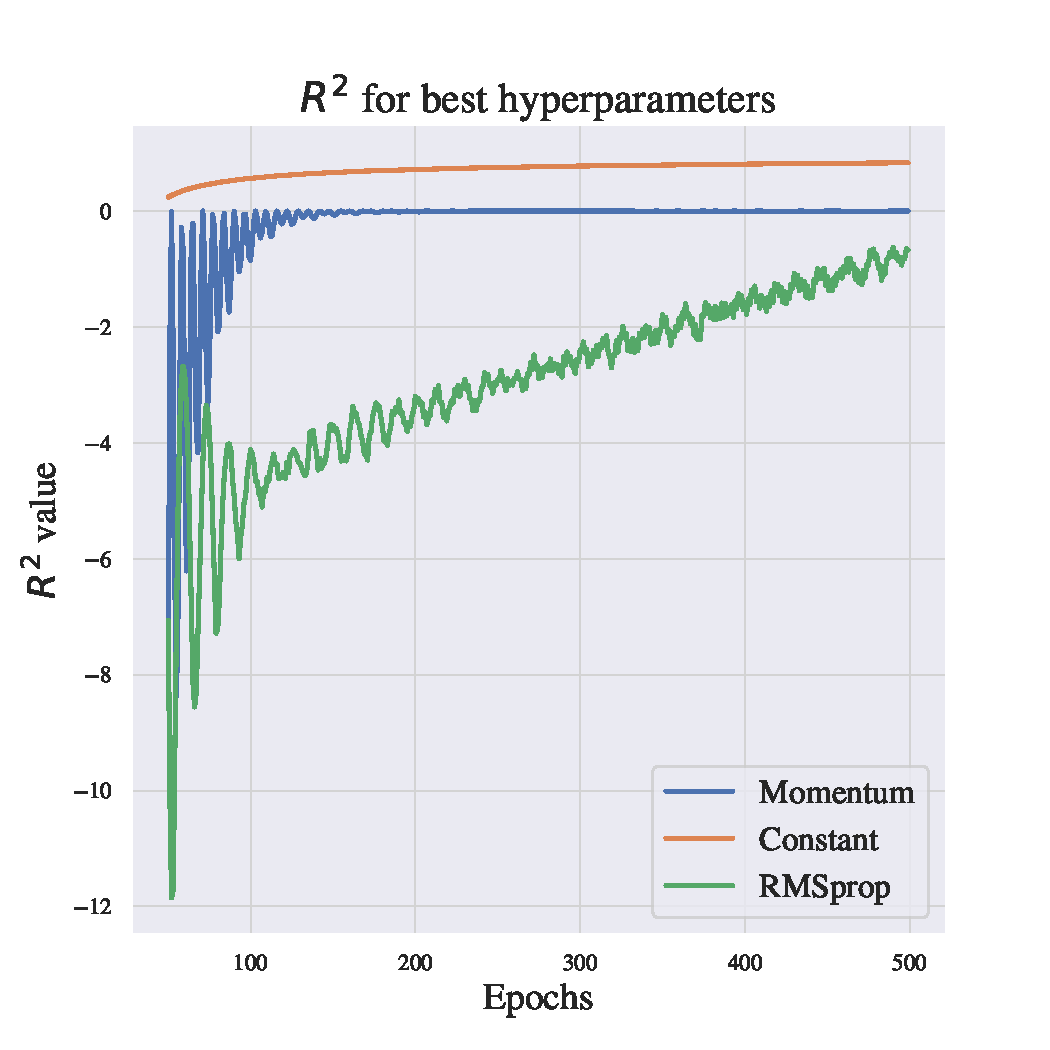
\includegraphics[width=1.0\linewidth]{project_2/figures/best_continuous.pdf}
    \caption{Caption}
    \label{fig:best_franke}
\end{figure}

The best model reaches an $R^2$ score of 0.77. This model is trained with the constant optimizer. 

\subsubsection{Linear regression}

Final values: 0.374

\subsection{Breast cancer data}

\subsubsection{Neural network}

Based on the initial search, using the Adam optimizer seems to be a good choice for the further investigation. The optimizers RMSprop and Adagrad with momentum make up the best three together with Adam. 

\begin{figure}[h!]
    \centering
    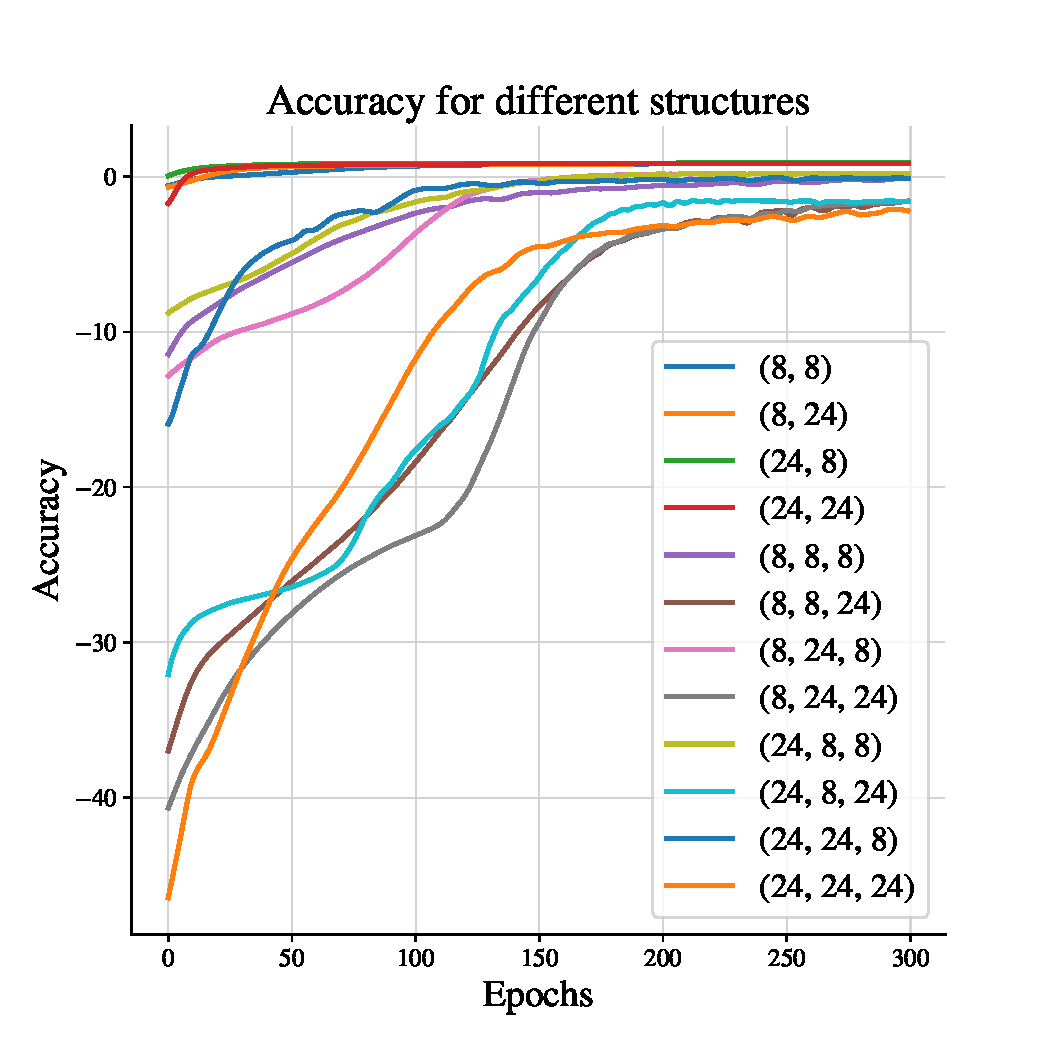
\includegraphics[width=1.0\linewidth]{project_2/figures/Accuracy for different structures_classification.pdf}
    \caption{$R^2$ for the neural network for different number of layers and sizes for each layer.}
    \label{fig:structure_cancer}
\end{figure}

Using the Adam optimizer, we test for the best structure of the network. As with the regression problem, two hidden layers are preferred over three. 
The best performing network, the one which gives the highest accuracy, is the one with (24, 8) as the hidden layers. The four best ones are the ones with only two layers, clearly shown on Fig. \ref{fig:structure_cancer}. The majorly outperform the models with three hidden layers. 
The reason for this might be \mia{}.

\begin{figure}[h!]
    \centering
    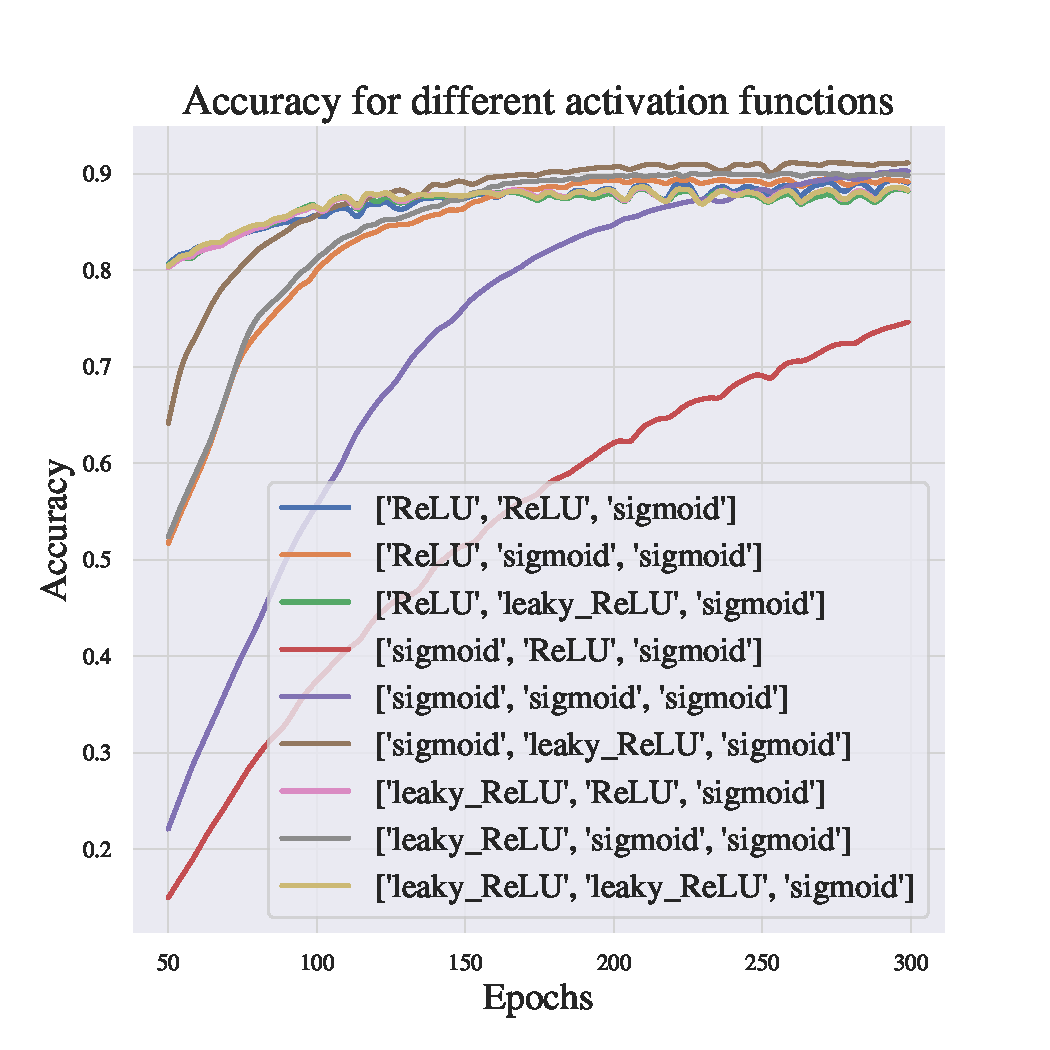
\includegraphics[width=1.0\linewidth]{project_2/figures/Accuracy for different activation functions_classification.pdf}
    \caption{Caption}
    \label{fig:activations_cancer}
\end{figure}

For these two hidden layers of size (24,8), Fig. \ref{fig:activations_cancer} shows how different choices of activation functions for the hidden layers lead to different accuracies. 
Sigmoid is always used as the activation function as the final layer. 
The best model is the one with (sigmoid, leaky ReLU) at the hidden layers. 
However, all seem to perform fairly well. \mia{more}

\begin{figure}[h!]
    \centering
    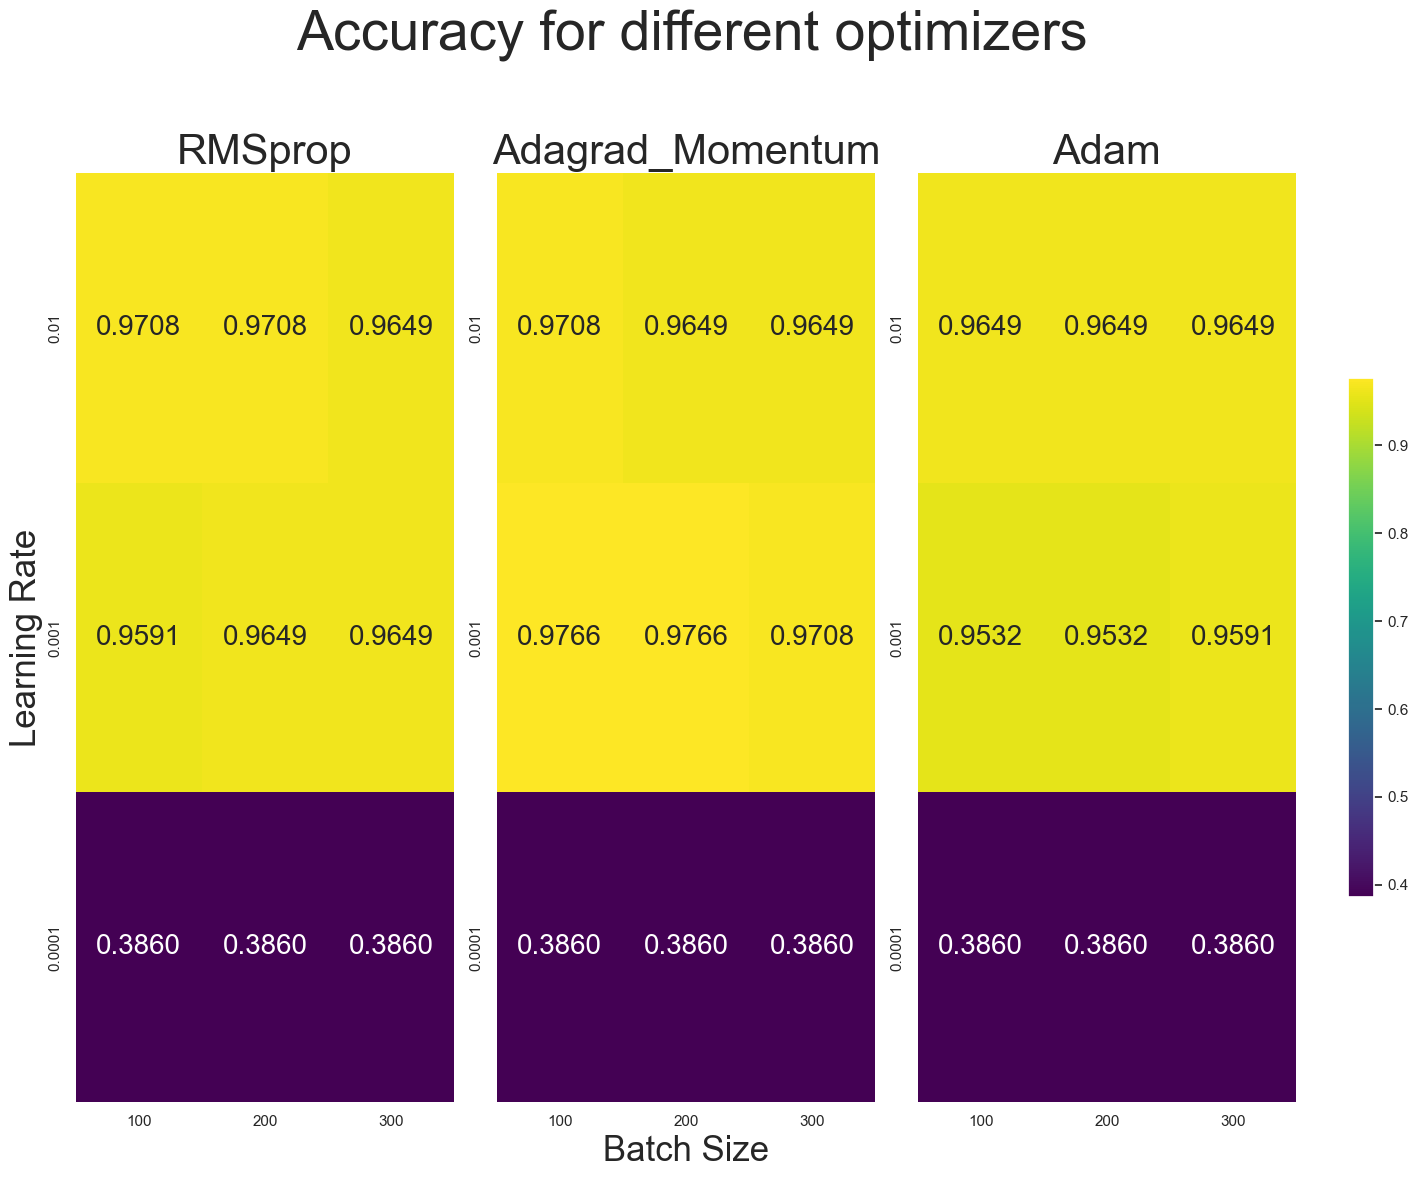
\includegraphics[width=1.0\linewidth]{project_2/figures/acc_grid_clas.png}
    \caption{\mia{terrible fig, must fix}}    
    \label{fig:grid_cancer}
\end{figure}

Given a network structure of (30,24,8,1) and (sigmoid, leaky ReLU, sigmoid) as the activation functions, we tested for the best combination of learning rate av batch size for each of the three best optimizers. Fig. \ref{fig:grid_cancer} shows how the lowest tested learning rate of 0.0001 yields very best accuracies regardless of optimizer and batch size. This might be because it has not yet converged within the maximal number of epochs. 
The results otherwise are very similar. \mia{more}

\begin{figure}[h!]
    \centering
    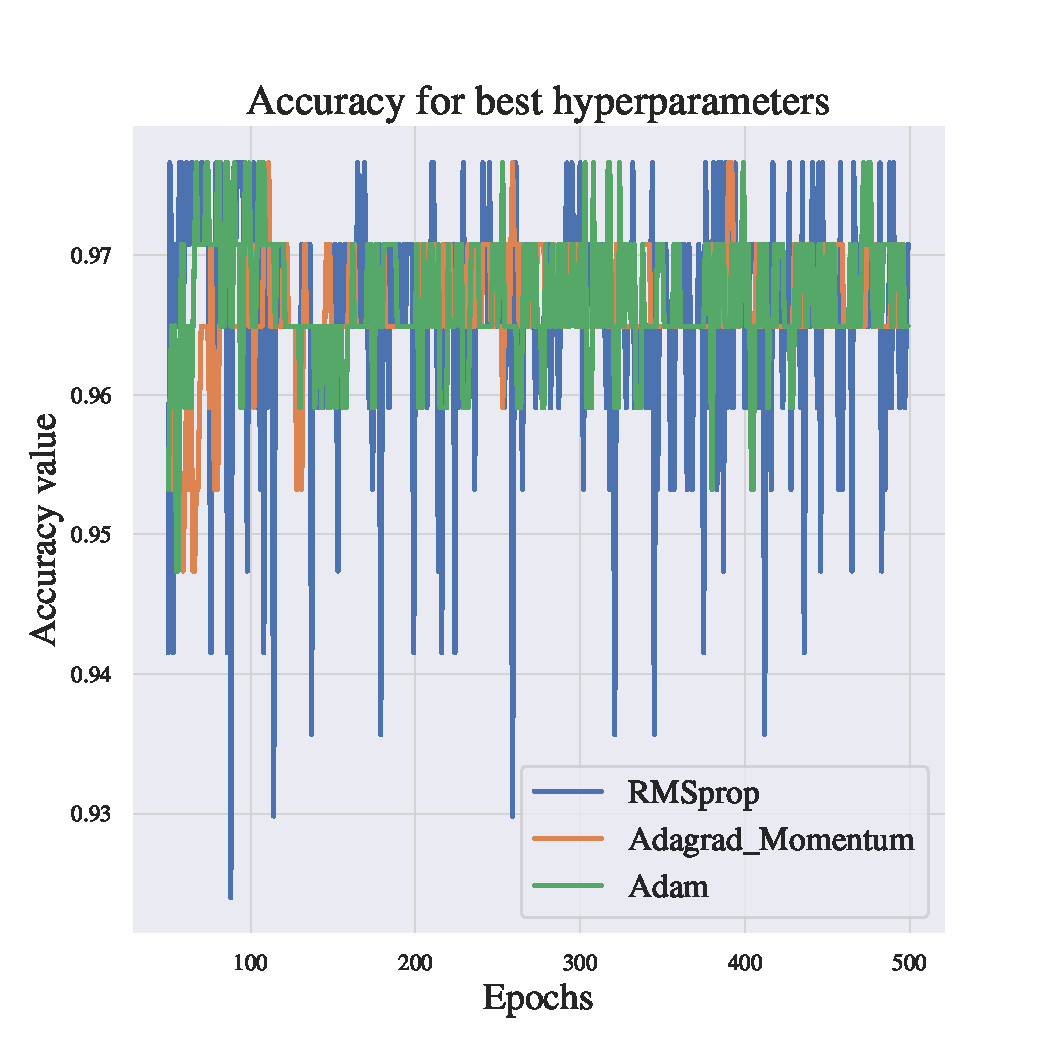
\includegraphics[width=1.0\linewidth]{project_2/figures/best_classification.pdf}
    \caption{\mia{cannot have this shit}}
    \label{fig:best_cancer}
\end{figure}

The best model for the classification problem given our method of exploring the different aspects, gives an accuracy of 0.97. 


\subsubsection{Logistic regression}

Our final logistic regression model has an accuracy of 0.97. This is the same as for the neural network \mia{double check later}.

We will consider the additional metrics recall, precision and F-score. In Tab. \ref{tab:class_score} \mia{bla bla}



\begin{table}[h]
    \centering
    \begin{tabular}{|m{8em}|m{8.5em}|m{8.5em}|}
    \hline
         & \textbf{NN} & \textbf{LogReg} \\
    \hline
        \textbf{Accuracy} & 0.97 & 0.97\\
    \hline
        \textbf{Precision} & 0.98 & 0.96 \\
    \hline
        \textbf{Recall} & 0.94 & 0.97 \\
    \hline
        \textbf{F-score} & 0.96 & 0.96 \\
    \hline
    \end{tabular}
    \caption{Scores for classification problem}
    \label{tab:class_score}
\end{table}



%Compare the results from the last project with the FFNN for regression tasks (can use Franke function)

%Compare the results from a logistic regression with the FFNN for classification tasks (breast cancer data)

%\mia{Desired plots:
%\begin{itemize}
%    \item Compare the gradient descent methods for OLS
%    \item Compare the gradient descent methods for Ridge
%    \item Compare results from FFNN to project 1 for OLS
%    \item Compare results from FFNN to project 1 for Ridge
%    \item compare logreg to ffnn for OLS and Ridge
%\end{itemize}}

%\mia{Needs discussion:\begin{itemize}
%    \item Learning rate $\eta$
%    \item Number of mini-batches 
%    \item Number of epochs 
%    \item For Ridge: the results as functions of $\lambda$
%    \item lin reg code from project 1 versus ffnn
%    \item critical discussion of pros and cons for each of the methods 
%\end{itemize}}